% !TEX program = pdflatex
\documentclass[xcolor=table]{beamer}

\usepackage[normalem]{ulem}
\usepackage{amsmath,amssymb}
\usepackage{graphicx}
\usepackage{tikz}
\usepackage{booktabs}
\usepackage{mathtools}

\newcommand{\ket}[1]{\lvert #1 \rangle}
\newcommand{\bra}[1]{\langle #1 \rvert}
\newcommand{\braket}[2]{\langle #1 \mid #2 \rangle}
\newcommand{\ketbra}[2]{\lvert #1 \rangle\!\langle #2 \rvert}
\newcommand{\proj}[1]{\ketbra{#1}{#1}}
\newcommand{\thinkingemoji}{%
  \tikz[baseline=-0.6ex, x=1ex, y=1ex]{
    \shade[ball color=yellow!80!orange] (0,0) circle (1);
    \fill (-0.33,0.24) circle (0.08);
    \fill (0.24,0.18) circle (0.08);
    \draw[line width=0.08ex] (-0.55,0.43) -- (-0.15,0.34);
    \draw[line width=0.08ex] (-0.18,-0.23) .. controls (0.03,-0.34) and (0.22,-0.24) .. (0.38,-0.12);
    \draw[line width=0.12ex, rounded corners=0.12ex] (0.08,-0.58) -- (0.54,-0.28) -- (0.44,-0.02);
  }%
}
\DeclareUnicodeCharacter{1F914}{\thinkingemoji}

\usetheme{Madrid}
\usecolortheme{default}
\setbeamertemplate{theorems}[numbered]
\setbeamertemplate{bibliography item}[text]
\newtheorem{claim}[theorem]{Claim}
\newtheorem{proposition}[theorem]{Proposition}
\newtheorem{observation}[theorem]{Observation}
\newtheorem{result}[theorem]{Result}
\theoremstyle{remark}
\newtheorem*{remark}{Remark}
\theoremstyle{plain}

% 하단 바: 이름(15%) | 제목(40%) | 섹션(35%) | 페이지(10%)
\setbeamertemplate{footline}{%
  \leavevmode%
  \hbox{%
    \begin{beamercolorbox}[wd=.15\paperwidth,ht=2.25ex,dp=1ex,center]{author in head/foot}%
      \usebeamerfont{author in head/foot}\insertshortauthor
    \end{beamercolorbox}%
    \begin{beamercolorbox}[wd=.40\paperwidth,ht=2.25ex,dp=1ex,center]{title in head/foot}%
      \usebeamerfont{title in head/foot}\insertshorttitle
    \end{beamercolorbox}%
    \begin{beamercolorbox}[wd=.35\paperwidth,ht=2.25ex,dp=1ex,center]{date in head/foot}%
      \usebeamerfont{date in head/foot}\insertsectionhead
    \end{beamercolorbox}%
    \begin{beamercolorbox}[wd=.10\paperwidth,ht=2.25ex,dp=1ex,right]{title in head/foot}%
      \insertframenumber{} / \inserttotalframenumber\hspace*{2ex}
    \end{beamercolorbox}}%
  \vskip0pt%
}

\setbeamertemplate{navigation symbols}{}
\setbeamercovered{transparent}

\pdfstringdefDisableCommands{%
  \def\\{ }%
}

\title[Quantum Min/Max Searching]{Quantum Min/Max Searching}
\subtitle{Lecture 3}
\author[Mingyu Lee]{Mingyu Lee\\{\small Seoul National University}}
\institute{\small red1108@snu.ac.kr\\+82 010-2857-3320 (only text) / +01 530-760-8690}
\date[2026.04.24(FRI) 16:30 KST]{2026.04.24(FRI) 16:30 KST}

\AtBeginSection[]
{
  \begin{frame}
    \frametitle{Outline}
    \tableofcontents[currentsection]
  \end{frame}
}

\begin{document}

\frame{\titlepage}

\begin{frame}
  \frametitle{Welcome back}
  Week 3. Thanks for coming back!

  \vspace{0.8em}
  Last two weeks we studied about \\
  
  \begin{itemize}
    \item Quantum Amplitude Amplification
    \item Quantum Amplitude Estimation
    \item Quantum Counting
  \end{itemize}

  This week we will see more practical applications of these primitives.
  \vspace{0.8em}
  \begin{itemize}
    \item Exponential searching (BBHT): Grover when $t$ is unknown
    \item D\"urr--H\o yer minimum-finding algorithm, $O(\sqrt{N})$
    \item Extension: find $k$ smallest items in $O(\sqrt{kN})$
  \end{itemize}

  \vspace{0.8em}
  All slides remain on GitHub: \url{https://github.com/red1108/lectures}
\end{frame}

\begin{frame}
  \frametitle{Outline}
  \tableofcontents
\end{frame}

\section{Motivation}

\begin{frame}
  \frametitle{Grover Recap}
  \begin{itemize}
    \item Given $f:\{0,1\}^n \to \{0,1\}$ and the promise that at least one $x$ satisfies $f(x)=1$
    \item Grover finds such $x$ in $O(\sqrt{N})$ queries, where $N=2^n$
    \item Classically we need $\Theta(N)$, and BBBV shows $\sqrt{N}$ is optimal
  \end{itemize}

  \vspace{0.5cm}
  \textbf{Now, instead of ``marked or not'', let's learn an algorithm that finds the min/max!}
\end{frame}

\begin{frame}
  \frametitle{Finding the Minimum}
  \begin{center}
    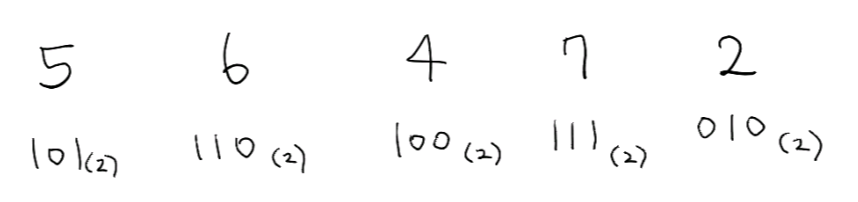
\includegraphics[width=\textwidth,keepaspectratio]{imgs/min_intro.png}
  \end{center}
\end{frame}

\begin{frame}
  \frametitle{From Search to Optimization}
  \begin{itemize}
    \item Problem: given values $T[0],\dots,T[N-1]$, find
      \[
        y^* = \arg\min_{0 \le y \le N-1} T[y]
      \]
    \item Classically: $\Theta(N)$ comparisons are necessary and sufficient
    \item Quantum question: can we do it in $O(\sqrt{N})$?
  \end{itemize}

  \vspace{0.5cm}
  \textbf{Yes.} D\"urr and H\o yer (1996) gave a surprisingly short algorithm\,\cite{durr1996minimum}.

  \vspace{0.3cm}
  The paper is only \textbf{2 pages long}.
\end{frame}

\begin{frame}
  \frametitle{Today's Algorithm}
  \begin{center}
    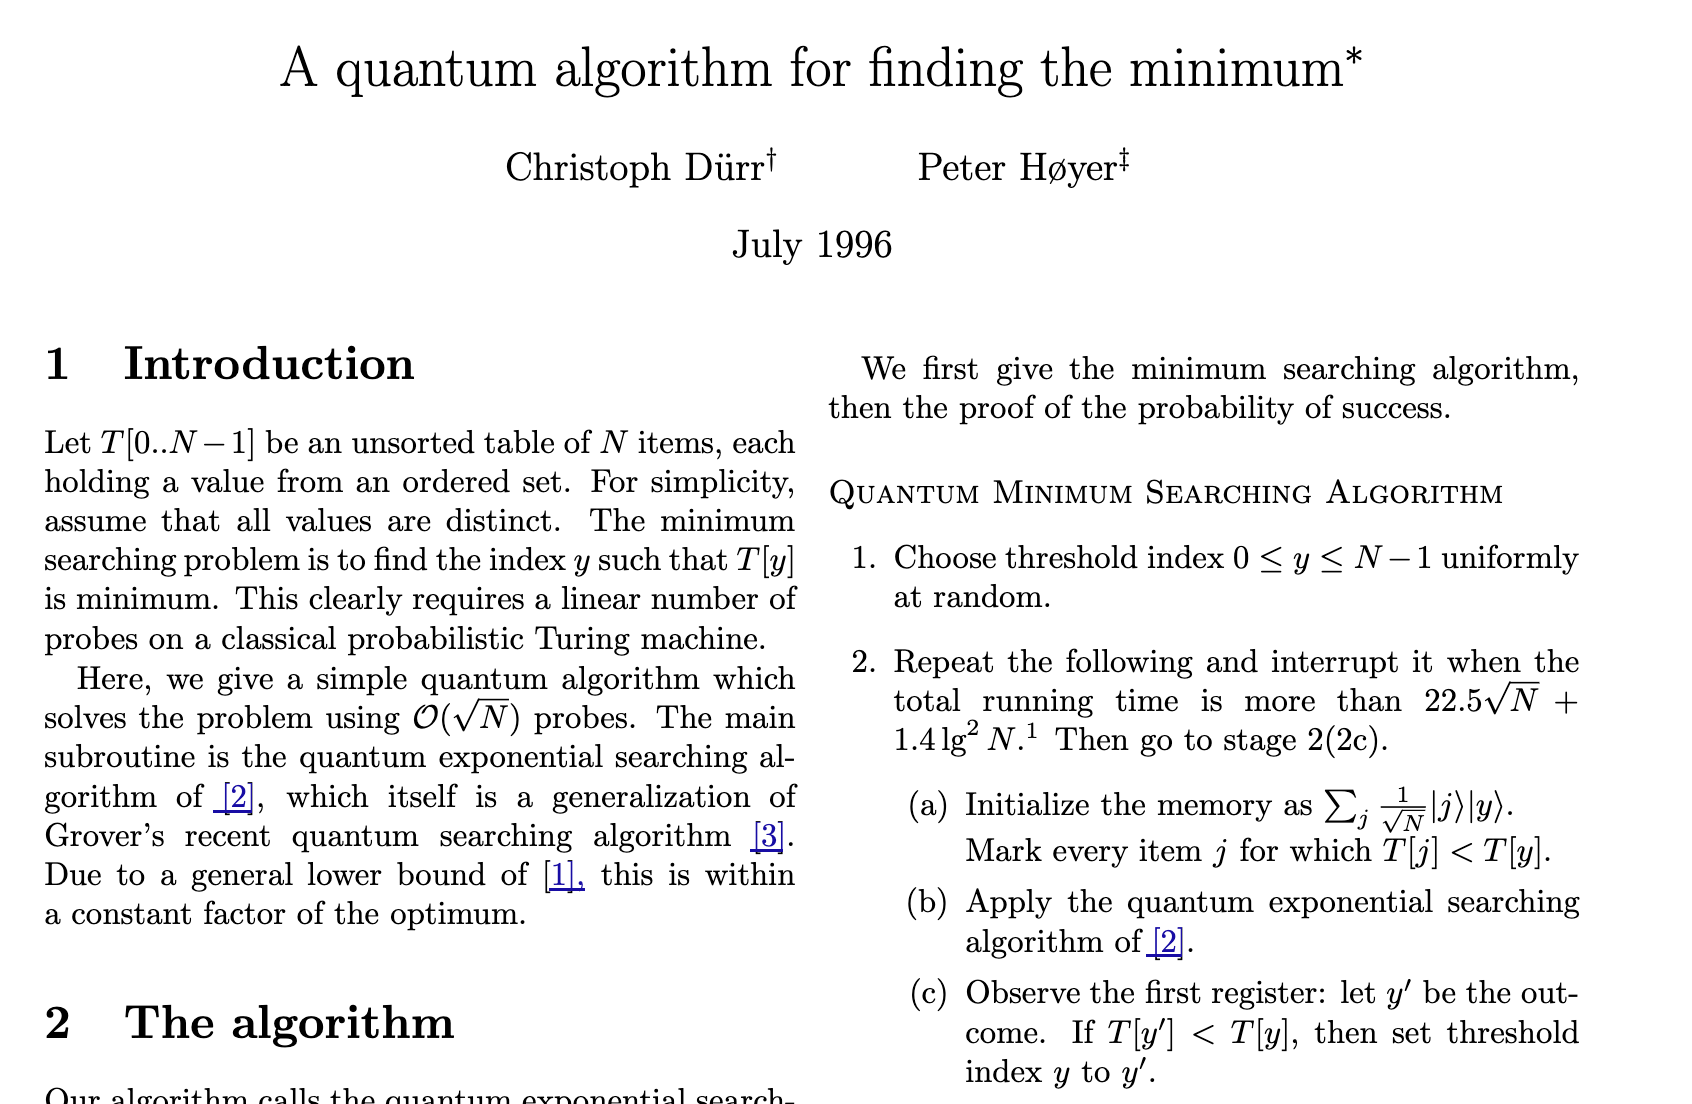
\includegraphics[width=0.8\textwidth,height=0.78\textheight,keepaspectratio]{imgs/algo1_abstract.png}
  \end{center}

  \vspace{-0.2cm}
  \begin{center}
    \textbf{This is what we will learn today.}
  \end{center}
\end{frame}

\begin{frame}
  \frametitle{Why Min Finding Matters}
  \begin{itemize}
    \item It is one of the simplest non-trivial quantum building blocks
    \item Appears as a subroutine in many algorithms:
    \begin{itemize}
      \item $k$-nearest neighbor
      \item clustering, classification
      \item shortest path, MST on graphs
    \end{itemize}
  \end{itemize}

  \vspace{0.5cm}
  \textbf{It is a simple application of Grover.}
\end{frame}

\section{Quantum Exponential Searching}

\begin{frame}
  \frametitle{Why Use Exponential Searching?}
  Recall how Grover works.

  \vspace{0.4cm}
  \begin{itemize}
    \item To find a marked item with high probability, we apply near $\left\lfloor \tfrac{\pi}{4}\sqrt{N/t}\, \right\rfloor$ Grover iterations, where $t$ is the number of marked items.
    \item Grover assumes we \textbf{know $t$ in advance}.
  \end{itemize}

  \vspace{0.5cm}
  \textbf{So we would first have to estimate $t$ with quantum counting (runs in $O(\sqrt{N})$, lecture 2) and then feed it into Grover.}
\end{frame}

\begin{frame}
  \frametitle{Two Ways to Handle Unknown $t$}
  There are two ways to run Grover without knowing $t$.

  \vspace{0.5cm}
  \begin{itemize}
    \item \textbf{Counting + Grover}: first guess $t$ with quantum counting, then run Grover.
    \item \textbf{Exponential searching}: works without knowing $t$.
  \end{itemize}

  \vspace{0.5cm}
  Both take the same time, $O(\sqrt{N/t})$ per call.

  \vspace{0.5cm}
  \textbf{Exponential searching is simpler. That is why most people use it as the subroutine.}
\end{frame}
\begin{frame}
  \frametitle{Quiz time!}
  \begin{center}
    
\includegraphics[width=0.8\textwidth,height=0.6\textheight,keepaspectratio]{imgs/survey_qr.png}
  \end{center}
\end{frame}

\begin{frame}
  \frametitle{Grover when $t$ Is Known}
  \begin{center}
    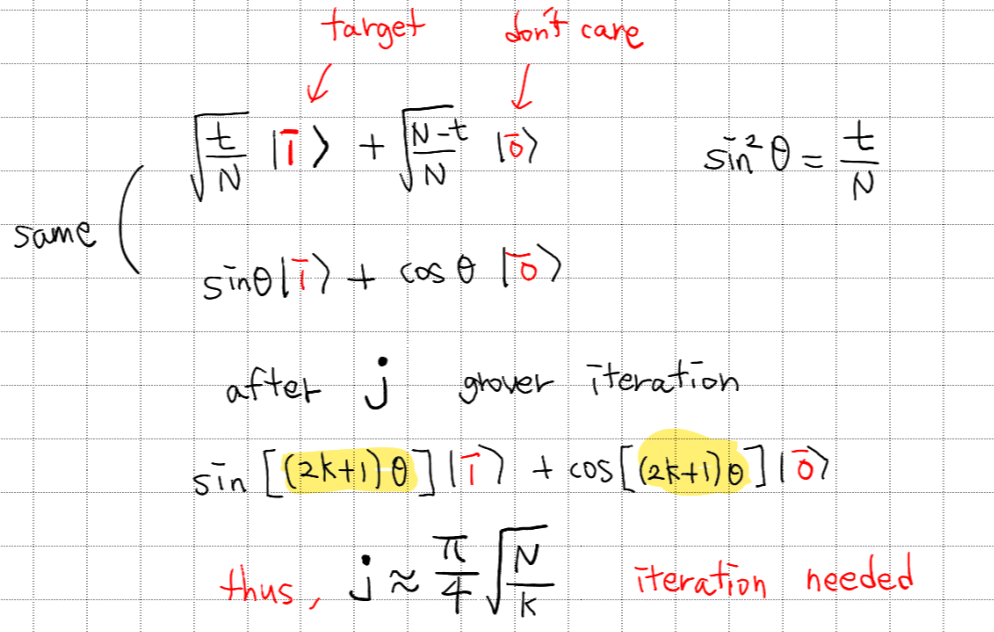
\includegraphics[width=\textwidth,height=0.82\textheight,keepaspectratio]{imgs/when_t_is_known.png}
  \end{center}
\end{frame}

\begin{frame}
  \frametitle{The Catch: $t$ Unknown}
  \begin{itemize}
    \item If we just use $m \approx \tfrac{\pi}{4}\sqrt{N}$ (good for $t=1$), the success probability is \textbf{not} monotone in $j$
    \item For $N = 2^{20}$ and $t = 1$, $m = 804$ iterations succeed almost certainly
    \item For $N = 2^{20}$ and $t = 4$, $m = 804$ iterations succeed with probability $< 10^{-6}$
  \end{itemize}

  \vspace{0.5cm}
  \textbf{The wrong $t$ drastically affects the success probability.}
\end{frame}

\begin{frame}
  \frametitle{The Averaging Trick}
  Idea: don't pick a single $j$, randomize over a window.

  \vspace{0.4cm}
  \begin{lemma}[BBHT, Lemma 2]
    Let $\sin^2\theta = t/N$ (unknown) and pick $j$ uniform in $\{0, \dots, m-1\}$. Apply $j$ Grover iterations and measure. Then
    \[
      P_m \;=\; \tfrac{1}{2} \;-\; \frac{\sin(4m\theta)}{4m\sin(2\theta)}.
    \]
    \textcolor{red}{\textbf{In particular, if $\boldsymbol{m \ge 1/\sin(2\theta)}$, then $\boldsymbol{P_m \ge 1/4}$.}}
  \end{lemma}

  \vspace{0.4cm}
  {\small Proof: average $\sin^2((2j+1)\theta)$ over $j$ via the cosine-sum identity.}
\end{frame}

\begin{frame}
  \frametitle{Lemma 1: Visual}
  \begin{center}
    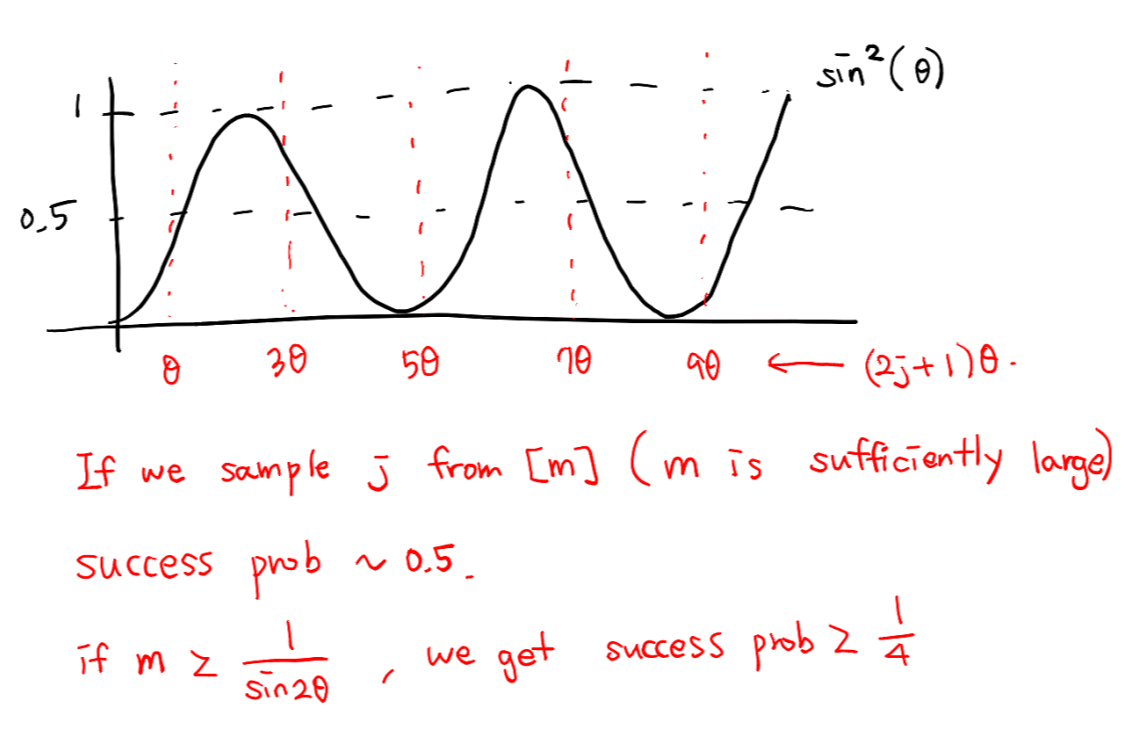
\includegraphics[width=\textwidth,height=0.82\textheight,keepaspectratio]{imgs/lemma1_explain.png}
  \end{center}
\end{frame}

\begin{frame}
  \frametitle{The BBHT Exponential Searching Algorithm}
  Inputs: oracle $f$, no knowledge of $t$. Choose any $\lambda \in (1, 4/3)$.

  \vspace{0.3cm}
  \begin{enumerate}
    \item Set $m \leftarrow 1$
    \item Pick $j$ uniformly at random in $\{0, \dots, m-1\}$
    \item Apply $j$ Grover iterations to the equal superposition; measure $i$
    \item If $f(i) = 1$, return $i$
    \item Else set $m \leftarrow \min(\lceil \lambda m \rceil, \sqrt{N})$ and go to step 2
  \end{enumerate}

  \vspace{0.4cm}
  \textbf{The window $m$ grows by a factor of $\lambda$ until it covers the critical scale
  $m_0 = 1/\sin(2\theta) \approx \tfrac{1}{2}\sqrt{N/t}$, where every round succeeds with probability $\ge 1/4$.}
\end{frame}

\begin{frame}
  \frametitle{BBHT Runtime}
  \begin{theorem}[BBHT, Theorem 3]
    For any $1 \le t \le 3N/4$, the algorithm returns a marked item in expected
    \[
      O\!\left(\sqrt{N/t}\right)
    \]
    Grover iterations, even though $t$ is unknown.
  \end{theorem}

  \vspace{0.4cm}
  Let $m_0 = 1/\sin(2\theta)$. Each round in round $s$ uses $m = \lceil \lambda^{s-1} \rceil$ as its window and costs $\tfrac{m}{2}$ Grover iterations on average.

  \vspace{0.3cm}
  \begin{itemize}
    \item \textbf{Phase 1 (ramp-up)}: $m$ grows by factor $\lambda$ until $m \ge m_0$.
      Geometric sum gives total cost
      $\;\le\; \dfrac{1}{2}\cdot\dfrac{\lambda}{\lambda - 1}\, m_0$
    \item \textbf{Phase 2 (critical stage)}: each round succeeds with prob.\ $\ge 1/4$.
      The dominant (last) round has cost
      $\;\le\; \dfrac{\lambda}{8 - 6\lambda}\, m_0$
  \end{itemize}
\end{frame}

\begin{frame}
  \frametitle{Plugging in $\lambda$}
  Adding the two phases,
  \[
    (\text{expected iterations}) \;\le\; C(\lambda)\, m_0,
    \qquad
    C(\lambda) \;=\; \frac{1}{2}\cdot\frac{\lambda}{\lambda - 1} \;+\; \frac{\lambda}{8 - 6\lambda}.
  \]

  \vspace{0.5cm}

  Now, substitute $C(6/5) = \frac{9}{2}$.

  \vspace{0.5cm}
  Using $m_0 \le \sqrt{N/t}$ (valid for $1 \le t \le 3N/4$):

  \vspace{0.3cm}
  \textbf{The algorithm uses at most $\tfrac{9}{2}m_0 \le \tfrac{9}{2}\sqrt{N/t}$ Grover iterations in expectation, with no prior knowledge of $t$.}
\end{frame}

\begin{frame}
  \frametitle{$C(\lambda)$ over $(1, 4/3)$}
  \begin{center}
    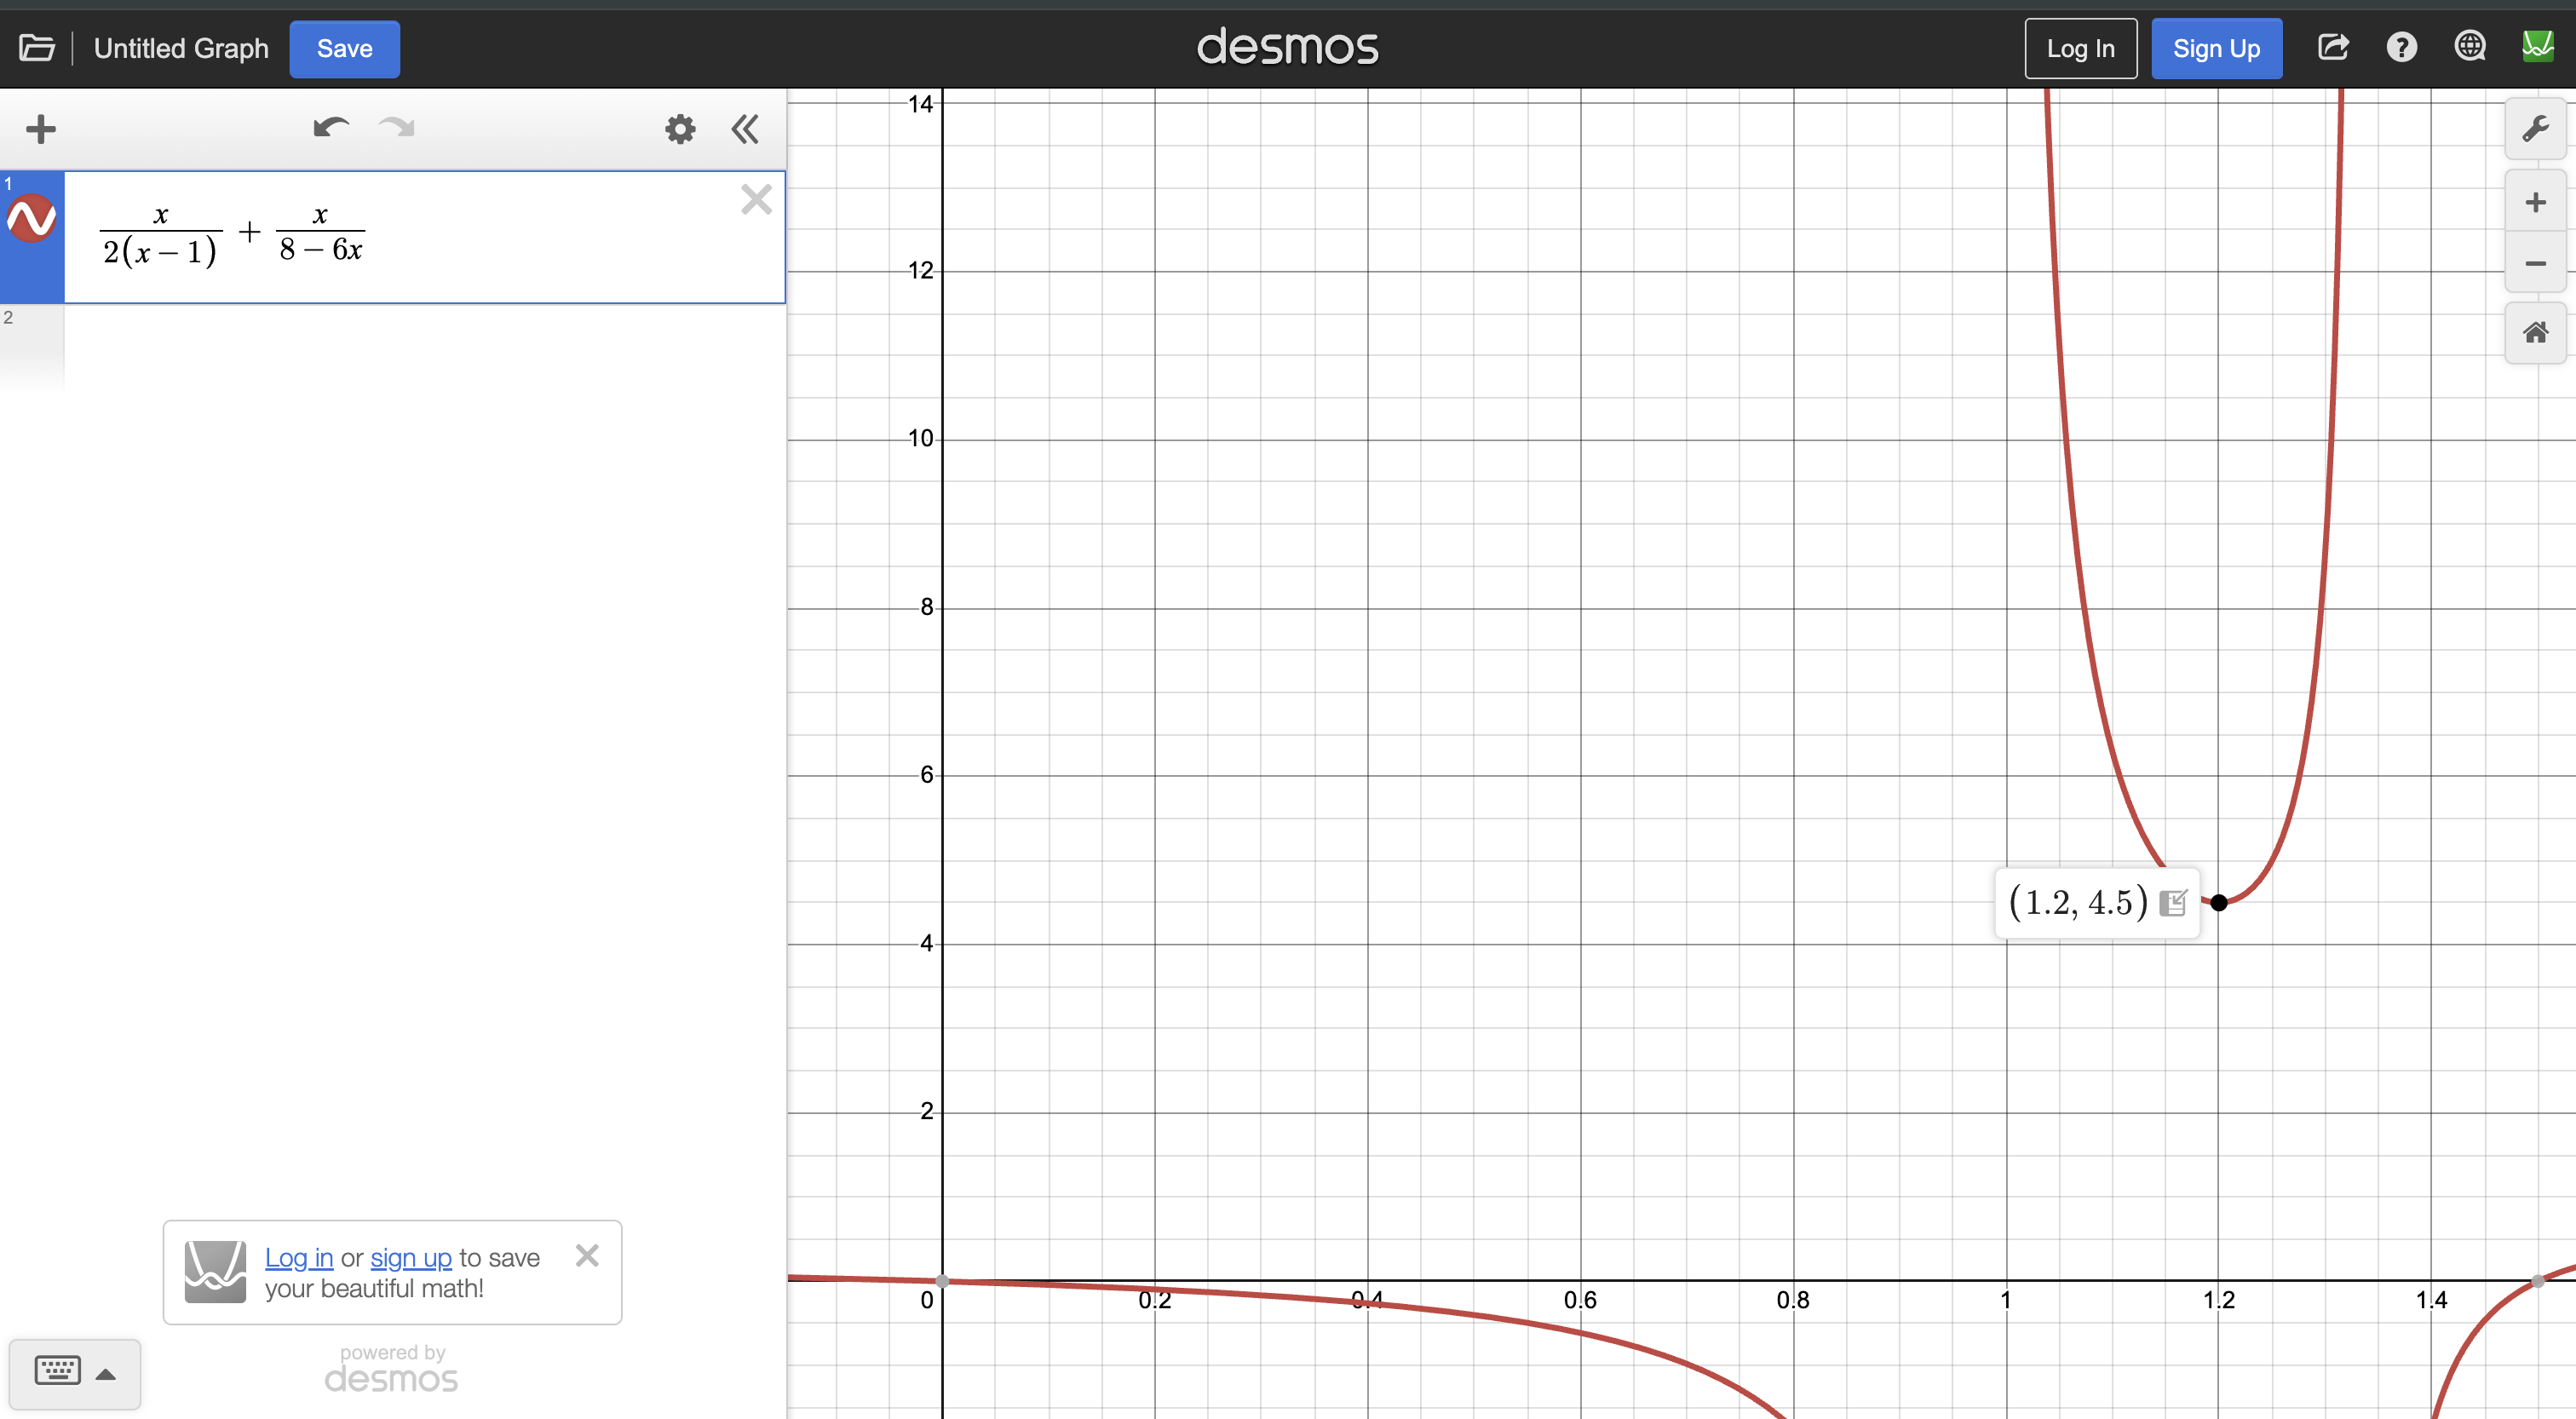
\includegraphics[width=\textwidth,height=0.7\textheight,keepaspectratio]{imgs/lambda_desmos.png}
  \end{center}

  \vspace{0.2cm}
  \begin{center}
    \textbf{We need at most $\tfrac{9}{2} m_0 \le \tfrac{9}{2}\sqrt{N/t}$ Grover iterations.}
  \end{center}
\end{frame}

\begin{frame}
  \frametitle{What About $t = 0$?}
  \begin{itemize}
    \item If no item is marked, this algorithm never halts.
    \item The ramp-up gets stuck at $m = \sqrt{N}$.
    \item At $m = \sqrt{N}$, \emph{if} there were even one marked item ($t \ge 1$), it should find it with probability $\ge 1/4$.
    \item We can just set the \textbf{time-out} as $r$.
    \item The false-negative probability is at most $(3/4)^r$.
  \end{itemize}

\end{frame}

\begin{frame}
  \frametitle{Black-Box Interface}
  For the rest of the lecture, treat exponential searching as a primitive:

  \vspace{0.4cm}
  \begin{block}{$\textsc{ExpSearch}(f)$}
    Input: oracle $f$ on $\{0,\dots,N-1\}$ with $t \ge 1$ marked items.\\[0.3em]
    Output: a uniformly random marked index.\\[0.3em]
    Cost: $\tfrac{9}{2}\sqrt{N/t}$ expected Grover iterations.
  \end{block}

  \vspace{0.5cm}
  \textbf{Two facts we will use:}
  \begin{itemize}
    \item output is uniform over marked items
    \item each call is independent; cost depends only on the current $t$
  \end{itemize}
\end{frame}

\section{The Minimum Finding Algorithm}

\begin{frame}
  \frametitle{What We Will Cover}
  \textbf{Idea:} keep picking any element smaller than the current one.
  Eventually you land on the minimum.

  \vspace{0.6cm}
  Each ``pick a smaller one'' step is one call to $\textsc{ExpSearch}$.

  \vspace{0.6cm}
  \textbf{Total cost: $O(\sqrt{N})$ Grover iterations.}
\end{frame}

\begin{frame}
  \frametitle{Covered on the Whiteboard}
  \vspace{1.5cm}
  \begin{center}
    {\Large \textbf{This section is covered by handwriting.}}
  \end{center}
\end{frame}

% Full slides for this section preserved in min_finding_full.tex (not included)

\section{Finding $k$ Minima}

\begin{frame}
  \frametitle{The $k$-Minima Problem}
  \begin{definition}[$k$-minima]
    Given $T[0..N-1]$ and $k \le N$, return the indices of the $k$ smallest values.
  \end{definition}

  \vspace{0.5cm}
  \begin{itemize}
    \item Naive classical(heap): scan all $N$ items, keep the $k$ smallest $\Rightarrow O(N\log{k})$
    \item Advanced classical(median of medians, optimal): Worst case $O(N)$. \vspace{0.2cm}
    \item Naive quantum: run D\"urr--H\o yer $k$ times $\Rightarrow O(k\sqrt{N})$
  \end{itemize}
  \vspace{0.4cm}
  Can we do \textbf{better than $k\sqrt{N}$}?

  \vspace{0.4cm}

  \textbf{Yes:} $O(\sqrt{kN})$ is achievable and optimal.
\end{frame}

\begin{frame}
  \frametitle{The $k$-Minima Problem}
  \begin{center}
    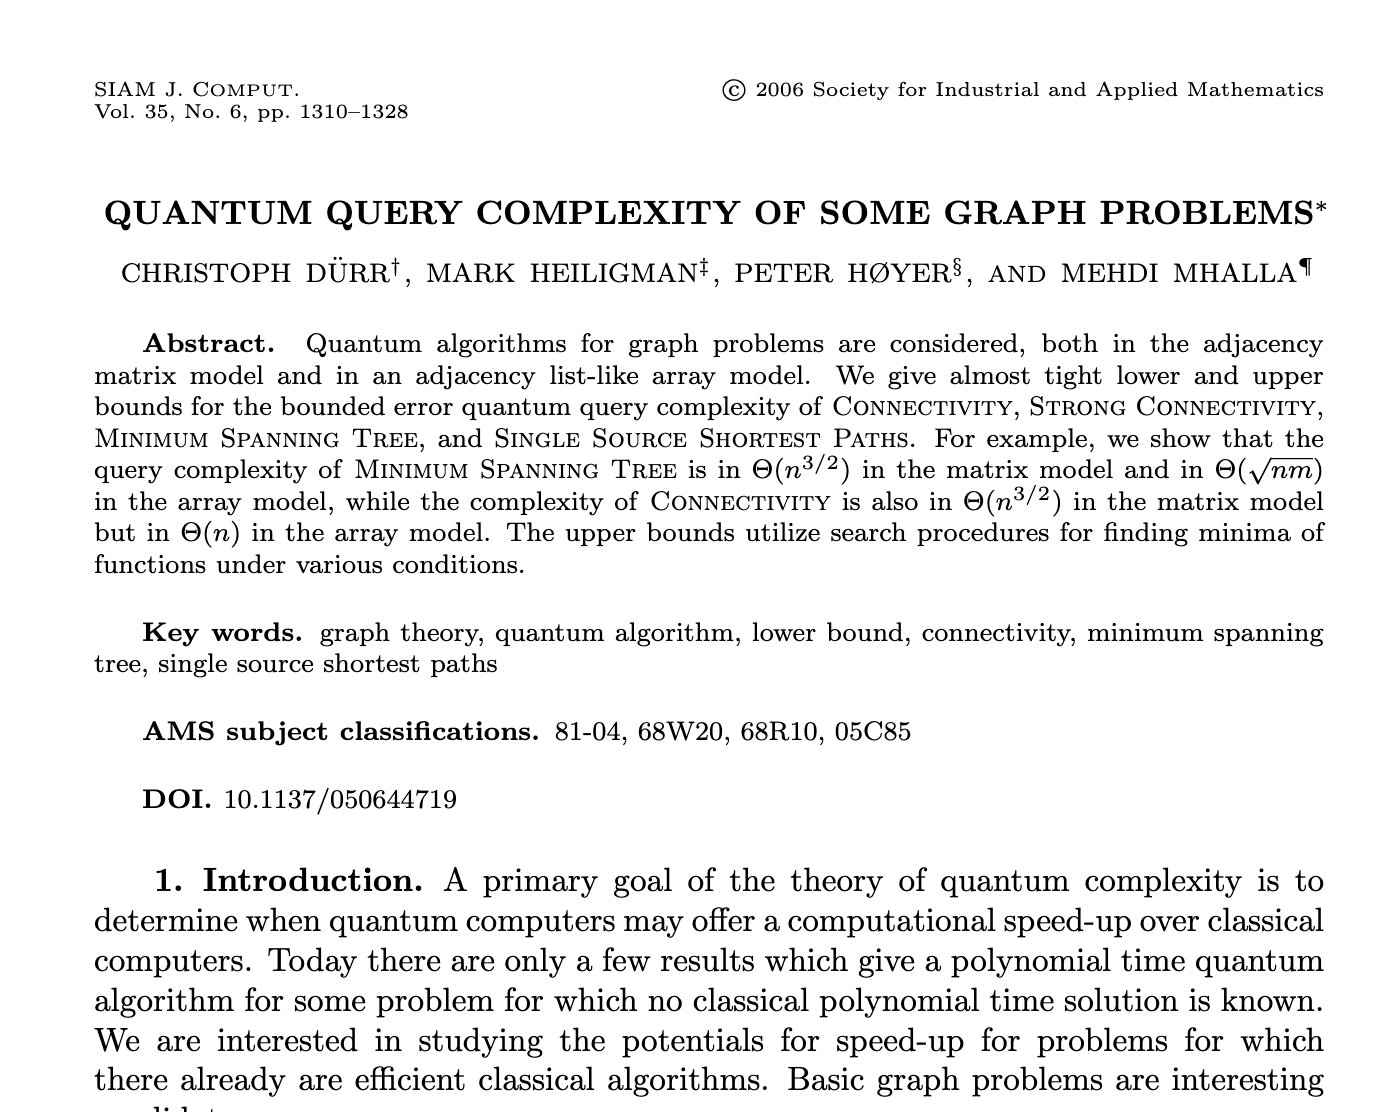
\includegraphics[width=\textwidth,height=0.5\textheight,keepaspectratio]{imgs/kminima_origin.png}
  \end{center}

  \vspace{0.2cm}
  The first $k$-minima algorithm was proposed in 2006\,\cite{durr2006quantum}, but the paper is 19 pages long... A simpler version appeared in 2019\,\cite{miyamoto2019kminima}.
\end{frame}


\begin{frame}
  \frametitle{A Well-Known Trick: $\sqrt{kN}$ Scaling}
  Think of finding marked items one by one:
  \[
    \underbrace{\sqrt{N/k}}_{\text{1st}} + \underbrace{\sqrt{N/(k-1)}}_{\text{2nd}} + \cdots + \underbrace{\sqrt{N}}_{k\text{-th}}
  \]

  \vspace{0.3cm}
  Bound the sum by an integral:
  \[
    \sum_{t=1}^{k}\sqrt{\tfrac{N}{t}}
    \le \sqrt{N}\left(1 + \int_1^k t^{-1/2}\,dt\right)
    = O(\sqrt{kN}).
  \]

  \vspace{0.3cm}
  \textbf{Each find gets cheaper as $k$ shrinks; the sum telescopes into $\sqrt{kN}$.}
\end{frame}

\begin{frame}
  \frametitle{Step 1: Run the Finding-Minimum Algorithm}
  Run FM and \textbf{record every threshold update along the way}.

  \vspace{0.6cm}
  \begin{center}
    {\large
    $T[y_1] \;>\; T[y_2] \;>\; T[y_3] \;>\; \cdots \;>\; T[y_m]$
    }
  \end{center}

  \vspace{0.6cm}
  \begin{itemize}
    \item Each $y_i$ is a threshold that FM accepted at some round
    \item The values are \textbf{strictly decreasing} by construction
    \item Total length: $m = O(\sqrt{N})$ \quad{\small (the FM expected runtime)}
  \end{itemize}

  \vspace{0.5cm}
  \textbf{The chain is essentially a sorted ladder of candidate thresholds.}
\end{frame}

\begin{frame}
  \frametitle{Step 2: We Don't Need an Exact Threshold}
  \textbf{Goal:} find an index $i$ such that
  \[
    \bigl|\{\,x : T[x] < T[i]\,\}\bigr| \;=\; k.
  \]

  \vspace{0.4cm}
  But hitting exactly $k$ is unnecessary. It is enough to find $i$ with
  \[
    k \;\le\; k' \;\le\; c \cdot k
    \qquad \text{for some constant } c.
  \]

  \vspace{0.4cm}
  \begin{itemize}
    \item This means O(k') = O(k) is good enough.
    \item Why? Discuss later.
  \end{itemize}
\end{frame}

\begin{frame}
  \frametitle{Binary Search on the Threshold Ladder}
  Recall the FM ladder: $T[y_1] > T[y_2] > \cdots > T[y_m]$, $m = O(\sqrt{N})$.

  \vspace{0.5cm}
  Two endpoints to anchor the search:
  \begin{itemize}
    \item $T[y_m]$ is the \textbf{minimum} \quad $\Rightarrow$ \quad $rank(y_m)-1 = 0$
    \item $T[y_{m-k}]$ has at least $k$ items below it \quad $\Rightarrow$ \quad $rank(y_{m-k})-1 > k$
  \end{itemize}

  \vspace{0.5cm}
  So a good threshold sits somewhere in $\{y_{m-k}, \dots, y_{m}\}$.

  \vspace{0.5cm}
  \begin{itemize}
    \item Binary search over these $k$ candidates: $O(\log k)$ steps
    \item Each step calls quantum counting once: $O(\sqrt{N})$
    \item \textbf{Total: $O(\sqrt{N}\log k)$ to locate $t_{k'}$.}
  \end{itemize}
\end{frame}

\begin{frame}
  \frametitle{The Process}
  \begin{block}{Pseudocode}
  \begin{flushleft}
  \ttfamily
  \textbf{repeat}: \\
  \quad Run Phase 1 \quad $\rightarrow$ \ candidate threshold $t_{k'}$ \\
  \quad Estimate $k' = h(t_{k'})$ via quantum counting \\
  \quad \textbf{if} $k' \le c \cdot k$: \quad \textbf{break} \ (success) \\
  \quad \textbf{else}: \quad retry \\
  Run Phase 2 with threshold $t_{k'}$
  \end{flushleft}
  \end{block}

  \vspace{0.4cm}
  \begin{itemize}
    \item Phase 1 alone may overshoot; quantum counting checks the size
    \item Each retry is independent, so a constant number suffice w.h.p.
  \end{itemize}
\end{frame}

\begin{frame}
  \frametitle{Phase 2: Extract All $k'$ Marked Items}
  We have a threshold $t_{k'}$ with exactly $k'$ items below it.

  \vspace{0.5cm}
  Pull them out one by one:
  \begin{itemize}
    \item Run $\textsc{ExpSearch}(f_{t_{k'}})$ to get one marked index
    \item Unmark it (remove from the search space)
    \item Repeat until the marked set is empty
  \end{itemize}

  \vspace{0.5cm}
  After $k'$ rounds we have collected all $k'$ items.

  \vspace{0.6cm}
  \textbf{Total query complexity?}
\end{frame}

\begin{frame}
  \frametitle{Phase 2: Cost Analysis}
  Each call to $\textsc{ExpSearch}$ depends on the current marked count:
  \[
    \underbrace{\sqrt{N/k'}}_{\text{round 1}} \;+\; \underbrace{\sqrt{N/(k'-1)}}_{\text{round 2}} \;+\; \cdots \;+\; \underbrace{\sqrt{N/1}}_{\text{round } k'}
  \]

  \vspace{0.4cm}
  This is exactly the $\sqrt{kN}$ trick from before:
  \[
    \sum_{t=1}^{k'} \sqrt{\tfrac{N}{t}} \;=\; O(\sqrt{k'N}).
  \]

  \vspace{0.4cm}
  Since $k' = O(k)$ by Phase 1's guarantee:
  \[
    O(\sqrt{k'N}) \;=\; O(\sqrt{kN}).
  \]
\end{frame}

\begin{frame}
  \frametitle{Trimming $k'$ Down to $k$}
  Phase 2 returns $k' \ge k$ items. We only want the smallest $k$.

  \vspace{0.5cm}
  \begin{itemize}
    \item Once we have the $k'$ values in classical memory, just sort and pick the smallest $k$
    \item Worst case: $O(k' \log k')$ classical comparisons
    \item This is \textbf{classical} work --- not counted in query complexity
  \end{itemize}

  \vspace{0.5cm}
  \textbf{The query complexity is set by Phases 1 and 2.}
\end{frame}

\begin{frame}
  \frametitle{Final Complexity Analysis}
  \begin{center}
  \renewcommand{\arraystretch}{1.3}
  \begin{tabular}{@{}lll@{}}
    \toprule
    \textbf{Stage} & \textbf{Cost} & \textbf{Source} \\
    \midrule
    Phase 1: FM ladder        & $O(\sqrt{N})$        & D\"urr--H\o yer \\
    Phase 1: binary search    & $O(\sqrt{N}\log k)$  & QC, $\log k$ steps \\
    Phase 2: extract $k'$     & $O(\sqrt{kN})$       & $\sum_t \sqrt{N/t}$ \\
    Trim to $k$               & free                 & classical \\
    \bottomrule
  \end{tabular}
  \end{center}

  \vspace{0.6cm}
  \[
    O(\sqrt{N}) + O(\sqrt{N}\log k) + O(\sqrt{kN})
    \;=\; \boxed{\,O(\sqrt{kN})\,}
  \]

  \vspace{0.4cm}
  $\sqrt{kN}$ dominates because $\sqrt{k} \ge \log k$ for all $k \ge 1$.
\end{frame}

% \section{Applications and Wrap-up}

% \begin{frame}
%   \frametitle{Where Min / $k$-Min Show Up}
%   \begin{itemize}[<+->]
%     \item \textbf{$k$-nearest neighbor:} find $k$ closest points to a query under a distance oracle
%     \item \textbf{Clustering:} nearest-centroid assignments, Lloyd-style updates
%     \item \textbf{Graph problems:} minimum-weight edge, single-source shortest path
%     \item \textbf{Optimization inner loops:} any ``pick the best candidate'' step
%   \end{itemize}

%   \vspace{0.4cm}
%   \only<5->{\textbf{Min finding is a quadratic speedup you can drop into almost any loop.}}
% \end{frame}

% \begin{frame}
%   \frametitle{What to Take Away}
%   \begin{itemize}[<+->]
%     \item Min finding $= $ Grover with a shrinking marked set
%     \item Key design trick: the \textbf{threshold oracle}, not a new amplitude technique
%     \item Clean analysis hinges on a single identity: rank $r$ is hit with probability $1/r$
%     \item $k$-min extends the same idea, and becomes modular once we split threshold-finding from enumeration
%     \item All of this is \textbf{optimal} up to constants
%   \end{itemize}

%   \vspace{0.5cm}
%   \only<6->{\textbf{Next week: quantum analog-digital conversion and the swap test.}}
% \end{frame}

\begin{frame}
  \frametitle{Quiz time!}
  \begin{center}
    
\includegraphics[width=0.8\textwidth,height=0.6\textheight,keepaspectratio]{imgs/survey_qr.png}
  \end{center}
\end{frame}

\section{References}

\begin{frame}[allowframebreaks]{References}
  \nocite{*}
  \bibliographystyle{alpha}
  \bibliography{citation}
\end{frame}

\end{document}
